
\documentclass[12pt,a4paper]{report}

%\RequirePackage[margin=3.0cm,a4paper]{geometry}

\usepackage{amsmath,amssymb,amstext}
\usepackage{times}
\usepackage[T1]{fontenc} 
\usepackage[utf8]{inputenc} 
\usepackage[ngerman]{babel}
\usepackage{graphicx, xcolor} 
\usepackage[
        plainpages=false,
        pdfpagelayout=TwoPageRight,
        pdfborder={0 0 0},
        hyperfootnotes=false
    ]{hyperref}
\usepackage{setspace} %mit /onehalfspacing wird im Textein 1,5 facher Zeilenabstand verwendet
\usepackage{accents}
\usepackage{color, colortbl}

\parindent 0pt


\begin{document}
    \onehalfspacing
    
    \begin{titlepage}
        \centering
        \includegraphics[width=0.4\textwidth]{./LogoSoFar.png}\par\vspace{1cm}
        {\scshape \LARGE BWolf \\ \Large Eine webbasierte Plattform zur
            Einschreibung und Verwaltung des
            Empiriepraktikums an der FSU Jena\par}
        \vspace{1.5cm}
        {\huge\bfseries Dokumentation\par}
        \vspace{1.5cm}
        {\large\itshape Christoph Keiner, Matthias Reuse, Ingo Schäfer, Christoph Staudt\par}
        \vspace{1.0cm}
        {\large \today\par}
    \end{titlepage}

    \pagenumbering{Roman}
    \tableofcontents 
    \clearpage
    \pagenumbering{arabic}
    
    
    \chapter{Einleitung}
\label{chapter:introduction}

    \chapter{Anforderungsanalyse}
\label{chapter:requirements}    

	In diesem Kapitel werden die Anforderungen an die Plattform dargestellt.
	Zunächst wird in Abschnitt \ref{sec:systemrequirements} behandelt, wie ein Praktikumsmodul abläuft und welche Erfordernisse sich daraus für die einzelnen Teilnehmergruppen ergeben.
	Darauf folgt eine Beschreibung der Aufgaben des Verteilungsalgorithmus.
	Zuletzt werden die technischen Anforderungen an das System beschrieben.
	
	\section{Anforderungen an das System}
		\label{sec:systemrequirements}
		Gemäß der allgemeinen Aufgabenstellung aus Abschnitt \ref{sec:task} existieren verschiedene Sichtweisen auf das Systems.
		Zum einen die Sicht der Verantwortlichen für Praktikum und Kurse, zum anderen die der Studenten.
		Erstere teilt sich wiederum in den Blickwinkel der Dozenten der Kurse und der übergeordneten Verantwortlichen für das Empiriepraktikum, im Weiteren Administratoren genannt, auf.
		Im Folgenden werden zunächst die Anforderungen für Studenten, Dozenten und Administratoren anhand des chronologischen Ablaufs eines Praktikumsmoduls dargestellt.
		Anschließend wird nochmals für die jeweiligen Sichten eine kurze Übersicht gegeben, sowie weitere detailliertere Anforderungen genannt.\\
		
		Die Anforderungen sind durch ein Gespräch mit den Verantwortlichen für das Empiriepraktikum entstanden. 
		Nicht alle Anforderungen sind zwingend für die Funktion des Systems.
		Einige sind optionale Funktionalitäten.
		Es ist zu beachten, dass aus zeitlichen Gründen nicht alle Anforderungen im Rahmen des Projektes umgesetzt werden konnten.
		Sie werden der Vollständigkeit halber dennoch aufgeführt.
		
		\subsection{Ablauf eines Praktikumsmoduls}
			Ein Praktikum beginnt, indem die Administratoren, nachdem sie sich in einer Oberfläche angemeldet haben, ein neues Praktikumsmodul erstellen.
			Zu diesem Praktikumsmodul gehören neben generellen Informationen wie Name und Semester auch die besonderen Angaben, ab wann Studenten ihre Präferenzliste erstellen können und zu welchem Zeitpunkt die automatische Verteilung vorgenommen werden soll.
			Im Anschluss können die Dozenten, nachdem auch sie sich in einer entsprechenden Oberfläche angemeldet haben, ihre Kurse zu dem aktuellen Praktikumsmodul hinzufügen.
			Dabei sollen Kurse Angaben über Titel, Dozent, Teilnehmerzahl, Ort, Zeit, Beschreibung des Kurses und eine Literaturliste besitzen.
			Zusätzlich soll ein Kurs Informationen über den Lehrstuhl, sowie die Finanzierung erhalten, die jedoch nicht für Studenten einsehbar sein soll.
			Nachdem alle Dozenten ihre Kurse eingetragen haben, sollen die Administratoren die aktuelle Kursübersicht online stellen können, sodass jeder die Kurse einsehen kann.
			Besteht Interesse, das Empiriepraktikum in diesem Semester zu absolvieren, so sollen sich die Studierenden registrieren können.
			Nach der Registrierung können die Studenten ihre Präferenzliste erstellen und speichern.
			Dabei soll die Präferenzliste auch jederzeit vom Studierenden noch verändert werden können.
			Nach jeder Änderung soll die Präferenzliste des Student gespeichert werden.
			Nach Ablauf der zuvor von den Administratoren festgelegten Frist können die Studenten anhand ihrer aktuellen Version der Präferenzliste auf die Kurse automatisch verteilt werden.
			Diese Verteilung sollte möglichst gut sein, d.h. in Fall dieses Projekts eine möglichst gleichmäßige Verteilung der Studenten mit vorzugsweise geringer Varianz.
			Nach dieser Verteilung soll eine Nachbearbeitungsphase folgen, in der die Administratoren das Ergebnis der Verteilung bei Bedarf manuell ändern können.
			Nachdem das Ergebnis der Verteilung fixiert wurde, sollen alle beteiligten Studenten, Dozenten und Administratoren über das Ergebnis der Verteilung mittels einer E-Mail-Benachrichtigung informiert werden.
			Ab diesem Moment sollen die Teilnehmer jedes Kurses für jeden angemeldeten Benutzer sichtbar sein.
			Anschließend an diese Nachbearbeitungsphase, könnte sich optional eine Tauschphase anschließen, in der die Studenten selbstständig über eine geeignete Oberfläche ihre Kurse tauschen können.
			
		\subsection{Verschiedene Sichten im Überblick}
		\label{Sichten}
		
			\subsubsection{Sicht der Administratoren}
				Administratoren haben die Möglichkeit ein neues Praktikum zu erstellen.
				Dabei müssen sie Angaben über Name, Semester, Frist für die Anmeldung und Beginn der automatischen Verteilung festlegen.
				Sie sollen aktiv die Kursübersicht für das aktuelle Praktikum veröffentlichen können.
				Des Weiteren können Administratoren den Verteilungsalgorithmus in der Nachbearbeitungsphase erneut mit anderen Parametern starten und die Verteilungsergebnisse auch manuell verändern.
				Zusätzlich sollen Administratoren die angemeldeten Dozenten verwalten können, um z.B. Dozenten, die keine Kurse mehr anbieten, zu entfernen.
				Auch sollen die Administratoren Kurse als \glqq frei bleiben\grqq~ markieren können, sowie die maximale und minimale Teilnehmerzahl für alle Kurse fließend einstellen können, falls nötig.
				Die Administratoren sollen für Praktika auch die Möglichkeit erhalten, Filterfunktionen anzuwenden und sich so z.B. die Kurse nach Lehrstühlen sortiert anzeigen zu lassen.
			
			\subsubsection{Sicht der Dozenten}
				Ein Dozent soll die Möglichkeit haben, Kurse für das aktuelle Praktikum zu erstellen und sich seine Kurse älterer Praktika nochmals anzusehen, um sie als Vorlage für neue Kurse zu nutzen. 
				Für einen Kurs müssen sie folgendes angeben: Name, Titel, Dozenten, Zeit und Raum, Teilnehmerzahl, eine Kurzbeschreibung des Kurses, eine ausführliche Beschreibung und optional eine Literaturliste.
				Diese Angaben sind auch für Studenten einsehbar.
				Dabei kann die Teilnehmerzahl nur auf fünf oder zehn gesetzt werden.
				Nicht für Studenten einsehbar sind die Angaben über Lehrstuhl, Lehrauftrag und die Information, ob der Dozent das erste Mal ein Empiriepraktikum leitet.
				
				Der Inhalt von längeren Angaben wie der Beschreibung des Praktikums, soll in einer Textumgebung möglich sein, in der geeignete Textformatierung möglich ist.
				Außerdem sollen auch Bilder in die Beschreibung eingearbeitet werden können.
				Des Weiteren sollen Dozenten nur ihre eigenen Kurse editieren können.
				Nachdem die Studenten verteilt worden sind, sollen die Dozenten eine E-Mail mit den Studenten, die in ihrem Kurs sind, erhalten.
				
				%                \todo{Im Verlaufe des Semesters können Dozenten ihren Kurs in zwei Kurse aufteilen.}
		
		
			\subsubsection{Sicht der Studenten}
				Die Studenten sollen ohne Registrierung die Kursübersicht aufrufen können, sobald die Administratoren die Kursübersicht veröffentlicht haben.
				Nach der Registrierung sollen die Studenten bis zu einer Frist eine Präferenzliste erstellen und späterhin auch bearbeiten können.
				Bei jeder angenommenen Änderung der Präferenzliste soll der Student über seine aktuelle Wahl per E-Mail informiert werden.
				Nachdem die Verteilung vom Algorithmus vorgenommen wurde, sollen die Studenten über ihr Ergebnis informiert werden, sowie die Ergebnisse der gesamten Verteilung einsehen können.
				Anschließend sollen sie eventuell die Möglichkeit erhalten, eigenständig die Kurse mit anderen Studenten zu tauschen, sofern beide zustimmen.
				
				
				%    	\todo{Das ganze offen und Modular halten für andere Module als das Empiriepraktikum}\\
				%    	\todo{Dabei auf Hierarchie von Präferenzen achten}\\
				%    	\todo{evtl. die Möglichkeit falls mehr Studenten als Kurse, neue Kurse hinzufügen können}\\
				%    	\todo{evtl. ein Archiv}\\
				%    
	
	
	
	\section{Der Verteilungsalgorithmus}
		Der Verteilungsalgorithmus verteilt alle Studenten auf die Kurse.
		Dabei ist es wichtig, dass die aufaddierte maximale Teilnehmeranzahl der Kurse größer ist als die Anzahl der zu verteilenden Studenten.
		Sollte dem nicht der Fall sein, so wird der Administrator informiert.
		Dieser hat nun die Möglichkeit die maximale Teilnehmeranzahl von Kursen zu erhöhen.
		Die Eingabe des Algorithmus sind die Gewichte der Präferenzen.
		
		Startet der Algorithmus, so versucht er, für jeden Studenten die größte, mögliche Präferenz zu den Kursen zu wählen.
		Dabei ist insbesondere wichtig, dass die Streuung der gewählten Präferenzen möglichst gering ist.
		Dies erfolgt beispielsweise durch eine Gewichtung der Präferenzen.\\
		Weiterhin platziert der Algorithmus in jeden Kurs mindestens drei Studenten, damit der Kurs sinnvoll angeboten werden kann.
		Es werden allerdings nie mehr Teilnehmer einem Kurs zugeordnet als die maximale Teilnehmeranzahl.
		
		Hat der Algorithmus schließlich eine passende Zuordnung von Studenten zu Kursen gefunden, so kann der Administrator die Ergebnisse bearbeiten, Parameter des Algorithmus neu einstellen, Kurse aktivieren/deaktivieren und ihn erneut starten.
		Ist der Administrator zufrieden mit der Verteilung, so bestätigt dieser das Ergebnis.
		Anschließend wird an die Dozenten eine E-Mail mit ihren Teilnehmern geschickt, und Studenten erhalten eine E-Mail mit ihrem Kurs.
		
	\section{Technische Details}
		
		Besucher der Website können sowohl auf mobilen Endgeräten, als auch per Desktop die Website besuchen.
		Diese passt sich dynamisch an die Bildschirmauflösung an.\newline
		Benutzt ein Besucher jedoch einen Browser, der älter als Internet Explorer 11 ist, so wird ihm mitgeteilt, er solle seinen Browser aktualisieren.\newline
		
		Der Login wird über eine E-Mail/Passwort Authentifizierung realisiert.
		Dafür sind nur E-Mail-Adressen der Friedrich-Schiller-Universität Jena nutzbar.
		Dies bedeutet, dass E-Mails auf \glqq @uni-jena.de\grqq~enden müssen.
		Die An- beziehungsweise Abmeldung ist hierbei zu jeder Zeit möglich.\newline
		
		Bei der Wahl der Präferenzen darf keine Präferenz doppelt belegt werden, d.h. jede Präferenz hat einen eindeutigen Kurs. \newline
		
		Der Verteilungsalgorithmus kann mit verschiedenen Optionen parametrisiert werden. Optionen können unter anderem die Gewichtung der Varianz, oder welche Kurse belegt werden können, sein. Weiterhin muss der Verteilungsalgorithmus innerhalb von 24 Stunden fertig sein. \newline
		
		Zu Zwecken der Portabilität wird das Produkt in einer docker-compose Umgebung ausgeführt.
		In dieser Umgebung soll die Website auf OctoberCMS mit Laravel 5.5 aufsetzen.
		Für den Webserver ist Nginx zu nutzen.
		Die Datenbank muss auf MySQL basieren.
		Zuletzt soll ein Cache-Server verwendet werden.
		Vorzugsweise ist dies Redis.\newline
		
		Die wesentlichsten Bestandteile der Website müssen über Tests validiert werden.
		Insbesondere der Verteilungsalgorithmus muss getestet werden.
		

    \definecolor{red}{rgb}{0.827,0.196,0.122}
\definecolor{orange}{rgb}{1.0,0.498,0.0}
\definecolor{olive}{rgb}{0.71,0.71,0.345}
\definecolor{green}{rgb}{0.118,0.490,0.216}
\definecolor{blue}{rgb}{0.447,0.624,0.812}

\chapter{Entwurf}
\label{chapter:design}
    Nachdem im vorangegangenem Kapitel die Anforderungen für das System spezifiziert wurden, soll in diesem Kapitel der Entwurf zur Umsetzung der Anforderungen der verschiedenen Sichten dargestellt werden.
    Zunächst wird das dem System zugrundeliegende Datenmodell dargestellt.
    Darauffolgend wird das Design für die webbasierte Plattform erläutert.     
    \section{Datenmodell}
        \begin{figure}
            \centering
            \includegraphics[width=1.0\textwidth]{./design/images/data-model.png}\par\vspace{1cm}
            \caption{Entwurf des Datenmodells}
            \label{fig:datamodel}
        \end{figure}
    
    \section{Design}
        Für den Desing-Entwurf der Seite wurden Mock-Ups erstellt, die den groben Aufbau der Website mit den entsprechenden Funktionen zeigt. 
        Im folgenden werden diese Mock-Ups für das sogenannte Frontend, also aus Sicht der Studenten, und für das Backend, die Sicht der Dozenten beziehungsweise der Administratoren, vorgestellt.
        Dabei gilt der in Tabelle \ref{tab:Farbcode} angegebene Farbcode für die verschiedenen Elemente der Mock-Ups.
        \begin{table}
            \centering
            \begin{tabular}{l c| l}
                \cellcolor{red} & & Eingabefeld\\
                \cellcolor{orange} & & Button\\
                \cellcolor{olive} & & Drag\&Drop-Element\\
                \cellcolor{green} & & Textfeld\\
                \cellcolor{blue} & & Optisches Element
            \end{tabular}
            \caption{Farbcode der Mock-Ups}
            \label{tab:Farbcode}
        \end{table}
    
        \subsection{Frontend}
            Wie in Kapitel \ref{chapter:requirements} bereits ausgeführt, sollen die Studenten zunächst eine Registrierungs- bzw. Login-Oberfläche sehen.
            Jedoch sollen die verschiedenen Kurse auch ohne eine Anmeldung einsehbar sein.
            \begin{figure}[t]
            	\centering
            	\includegraphics[width=0.7\textwidth]{./design/images/MockUpsFrontend/frontendLogin.png}
            	\caption{Entwurf für die Login-Oberfläche}
            	\label{mockupLoginFrontend}
            \end{figure}   
        
            In Abbildung \ref{mockupLoginFrontend} werden beide Anforderungen umgesetzt.
            Zum einen die Login-Oberfläche, in der in zwei Textfelder Benutzername und Passwort für einen erfolgreichen Login eingetragen werden müssen, zum anderen die direkte Weiterleitung zur Kursübersicht als einfacher Knopf darunter.

            Die Kopfzeile umfasst einige Reiter.
            So kann mithilfe der Kopfzeile auf die verschiedenen Funktionen des Frontends gewechselt werden. 
            Dazu zählen die Kursübersicht, die Erstellung der Präferenzliste, das Einsehen der Verteilungsergebnisse, sowie das Tauschen von Kursen.
            Außerdem soll in der Kopfzeile ein Schalter zum Abmelden aus dem System bereitgestellt werden und eine Anzeige, ab wann das Ende der Einschreibungs- und Tauschphase erreicht ist.
            Auf allen weiteren Seiten soll die Kopfzeile die gleiche Funktion und das gleiche Aussehen haben.
            Unter der Kopfzeile folgt eine textuelle Erklärung des Ablaufs des Empiriepraktikums und der für die Studenten relevanten Schritte, um sich erfolgreich für die Kurse einzuschreiben.
            Wie in Abbildung \ref{mockupCoursesFrontend} dargestellt, werden darunter die verschiedenen Kurse angezeigt, jeweils mit einer kurzen Beschreibung.
            Durch einen Klick auf ein Kursfeld, sollen sich die detaillierten Informationen zu dem Kurs einsehen lassen.
            Das Desing hierfür ist in Abbildung \ref{mockupDetailsFrontend} zu sehen und bedarf keiner weiteren Erläuterung.
            \begin{figure}[t]
            	\centering
            	\includegraphics[width=0.7\textwidth]{./design/images/MockUpsFrontend/frontendCoursedetails.png}
            	\caption{Entwurf für die Kursdetails}
            	\label{mockupDetailsFrontend}
            \end{figure}
            Die Fußzeile soll weitere allgemeine Informationen bereitstellen, sofern diese von Nöten sein sollten, aber vor allem als optischer Abschluss der Seite dienen.
            \begin{figure}[t]
            	\centering
            	\includegraphics[width=0.7\textwidth]{./design/images/MockUpsFrontend/frontendPreferences.png}
            	\caption{Entwurf für die Einschreibungs-Oberfläche}
            	\label{mockupPreferencesFrontend}
            \end{figure}
            
            Die Seite für die Einschreibung in die Kurse soll wie in Abbildung \ref{mockupPreferencesFrontend} gestaltet sein.
            Wieder bilden Kopfzeile und Fußzeile den Rahmen der Seite.
            Unter der Kopfzeile befindet sich auch hier eine kurze Erklärung, wie man die Präferenzliste genau erstellt.
            Das Erstellen soll im Feld \textit{Präferenzliste} über ein ''Drag\&Drop''-System vorgenommen werden und über den Knopf \textit{Absenden} fixiert werden können.
            
            \begin{figure}[t]
                \centering
                \includegraphics[width=0.7\textwidth]{./design/images/MockUpsFrontend/frontendSwap1.png}
                \caption{Entwurf für die Tauschauswahl}
                \label{mockupResultsFrontend}
            \end{figure}
        
            \begin{figure}[t]
                \centering
                \includegraphics[width=0.7\textwidth]{./design/images/MockUpsFrontend/frontendSwap2.png}
                \caption{Entwurf für die Tauschanfrage}
                \label{mockupResultsFrontend}
            \end{figure}
            
    
        \subsection{Backend}
        	\subsubsection{Administratoren}
        	\subsubsection{Dozenten}
    \chapter{Umsetzung}
\label{chapter:implementation}
    In diesem Kapitel wird die Umsetzung des System erläutert.
    Zunächst wird die zur Implementierung verwendete Software näher erläutert.
    Anschließend werden Front- und Backend kurz vorgestellt und mit dem Entwurf aus Kapitel \ref{chapter:design} verglichen.
    Zur Versionsverwaltung der verwendeten Komponenten wurde die GitHub Organisation BwolfJena\footnote{\href{https://github.com/BWolfJena}{https://github.com/BWolfJena}} erstellt.
    
    \section{Verwendete Software}

        Für die lokale Entwicklung wurde als Basis \textit{Laradock}\footnote{\href{http://laradock.io/}{http://laradock.io/}} verwendet und auf die benötigte Software angepasst.
        Diese modifizierte \textit{Laradock} Variante wurde als \textit{git submodule} in das Hauptrepository \textit{BWolf} eingebunden.
        Als Webserver kommt lokal \textit{nginx}\footnote{\href{https://nginx.org/en/}{https://nginx.org/en/}} zum Einsatz, wobei die \textit{PHP}\footnote{\href{http://php.net/}{http://php.net/}} \textit{7.1} Skripte von \textit{php-fpm}\footnote{\href{https://php-fpm.org/}{https://php-fpm.org/}} ausgeführt werden.
        In der Produktionsumgebung wird \textit{Apache} verwendet, weitere Details sind nicht bekannt.
        Für die Datenbank kommt in allen Umgebungen \textit{MySQL}\footnote{\href{https://www.mysql.com/de/}{https://www.mysql.com/de/}} zum Einsatz.
        Um auch lokal E-Mails verschicken und testen zu können, wird \textit{MailDev} als \textit{SMTP} Server verwendet.
        Für den Verteilungsalgorithmus wird \textit{Node.js 8}\footnote{\href{https://nodejs.org/en/}{https://nodejs.org/en/}} eingesetzt.
        
        Als Entwicklungsframework für \textit{PHP} wird \textit{October CMS}\footnote{\href{https://octobercms.com/}{https://octobercms.com/}} (basierend auf \textit{Laravel}\footnote{\href{https://laravel.com/}{https://laravel.com/}} 5.5.) verwendet. 
        Ein Großteil der Funktionalitäten, wie die Front- und Backendbenutzerverwaltung und die Inhaltsverwaltung werden dabei von \textit{October CMS} bereitgestellt. 
        Die Verwaltungsansichten werden basierend auf \textit{yaml} Dateien generiert. 
        Im Frontend kommt \textit{Semantic UI}\footnote{\href{https://semantic-ui.com/}{https://semantic-ui.com/}} \textit{2.2} zum Einsatz, wodurch die Webseite ohne größere Anpassungen auf Mobilgeräten komfortabel benutzt werden kann. 
        Schließlich dient das \textit{Express}\footnote{\href{http://expressjs.com/de/}{http://expressjs.com/de/}} \textit{Framework} als Basis für den Algorithmus Mini-HTTP Server (weitere Details in Kapitel \ref{chapter:algorithm}).                
    \section{Frontend}
        Die Entwürfe für das Frontend wurden ohne große Änderungen umgesetzt.
        
	        \begin{figure}[p]
	            \centering
	            \begin{subfigure}{\textwidth}
	            	\centering
	                \includegraphics[width=\textwidth]{./implementation/images/MockUpsFrontend/frontendLogin.png}
	            \end{subfigure}
	            \begin{subfigure}{\textwidth}
	                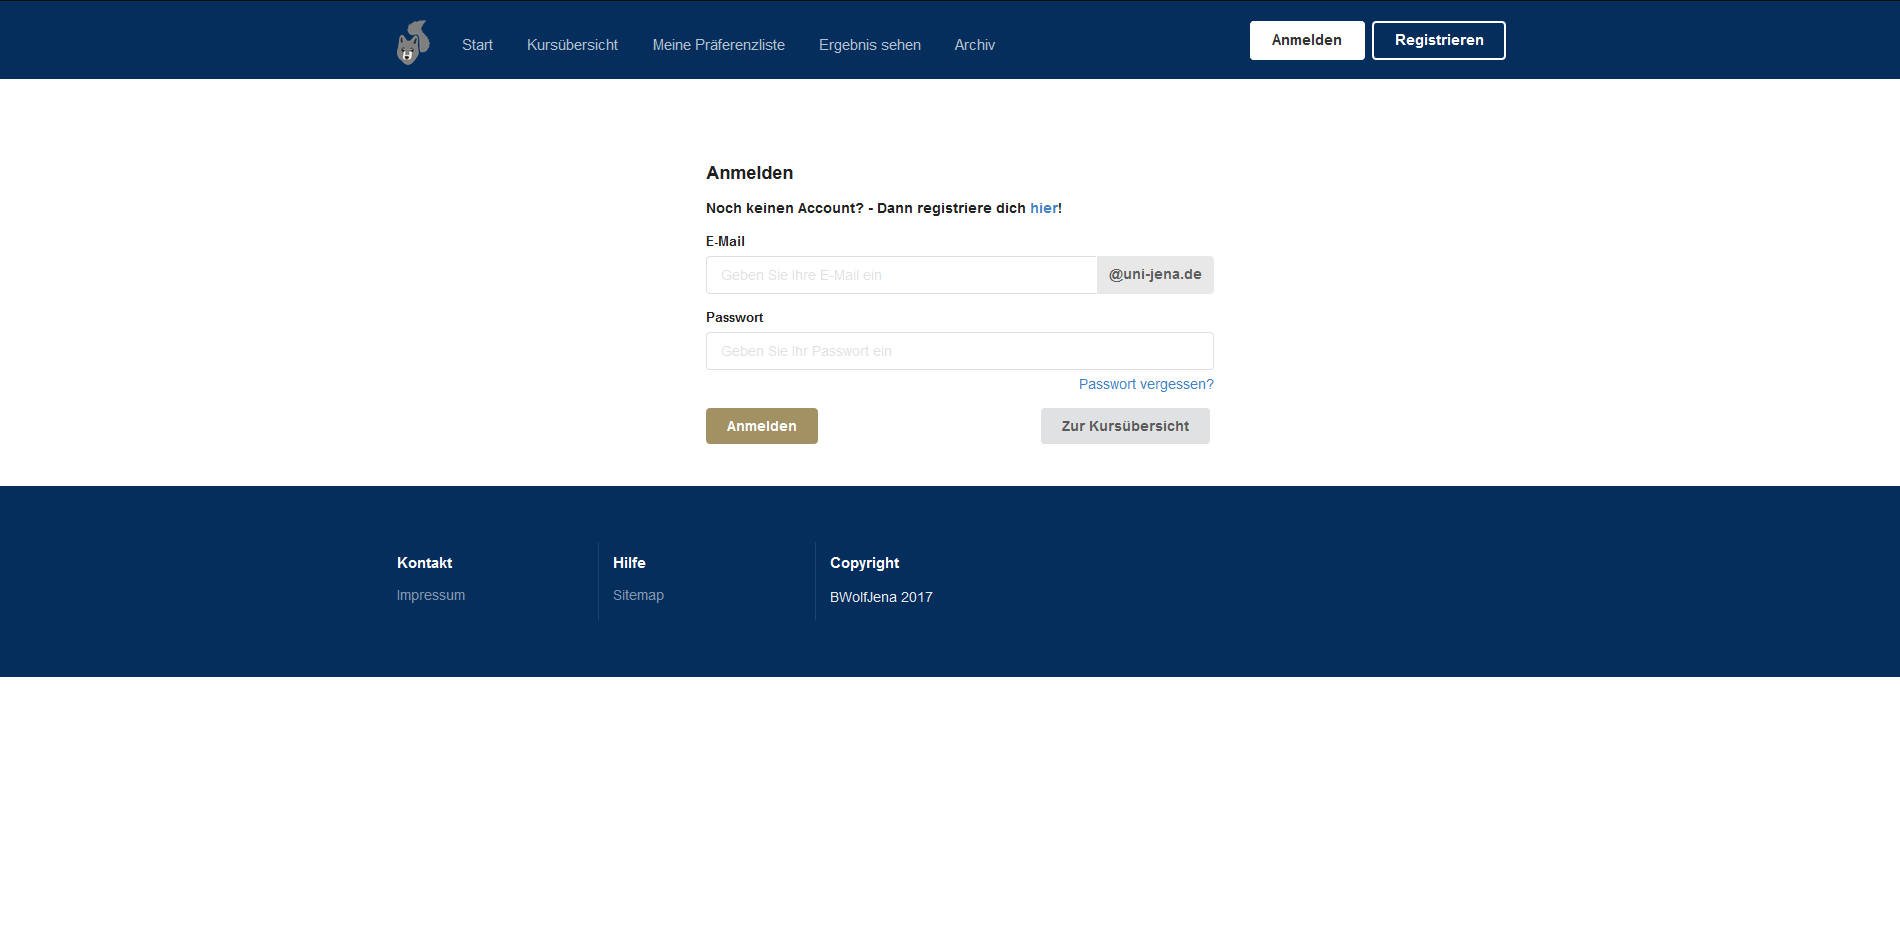
\includegraphics[trim={5cm 0 5cm 0}, clip, width=\textwidth]{./implementation/images/login.png}
	            \end{subfigure}
	            \caption{Gegenüberstellung von Entwurf der Login-Oberfläche und Umsetzung }
	            \label{fig:comparisonLogin}
	       \end{figure}
	    
    
        In Abbildung \ref{fig:comparisonLogin} sind der Entwurf für die Login-Oberfläche und die Umsetzung selbiger gegenüber gestellt.
        Es fällt auf, dass die grobe Struktur der Seite bis auf kleine Änderungen mit dem Entwurf übereinstimmt.
        Unterschiede lassen sich vor allem in der Kopfzeile erkennen.
        So wurde der Reiter \textit{Start} hinzugefügt.
        Anders als zuvor angedacht, fiel die Entscheidung für eine Startseite, in der das Empiriepraktikum kurz vorgestellt wird.
        Des Weiteren wurde der Reiter \textit{Einschreiben} aus Gründen der Verständlichkeit in \textit{Meine Präferenzliste} umbenannt.
        Die Seite erfüllt jedoch die selbe Funktion.
	        \begin{figure}[p]
	            \centering
	            \begin{subfigure}{\textwidth}
	                \includegraphics[width=1.0\textwidth]{./implementation/images/MockUpsFrontend/frontendCourses.png}
	            \end{subfigure}
	            \begin{subfigure}{\textwidth}
	                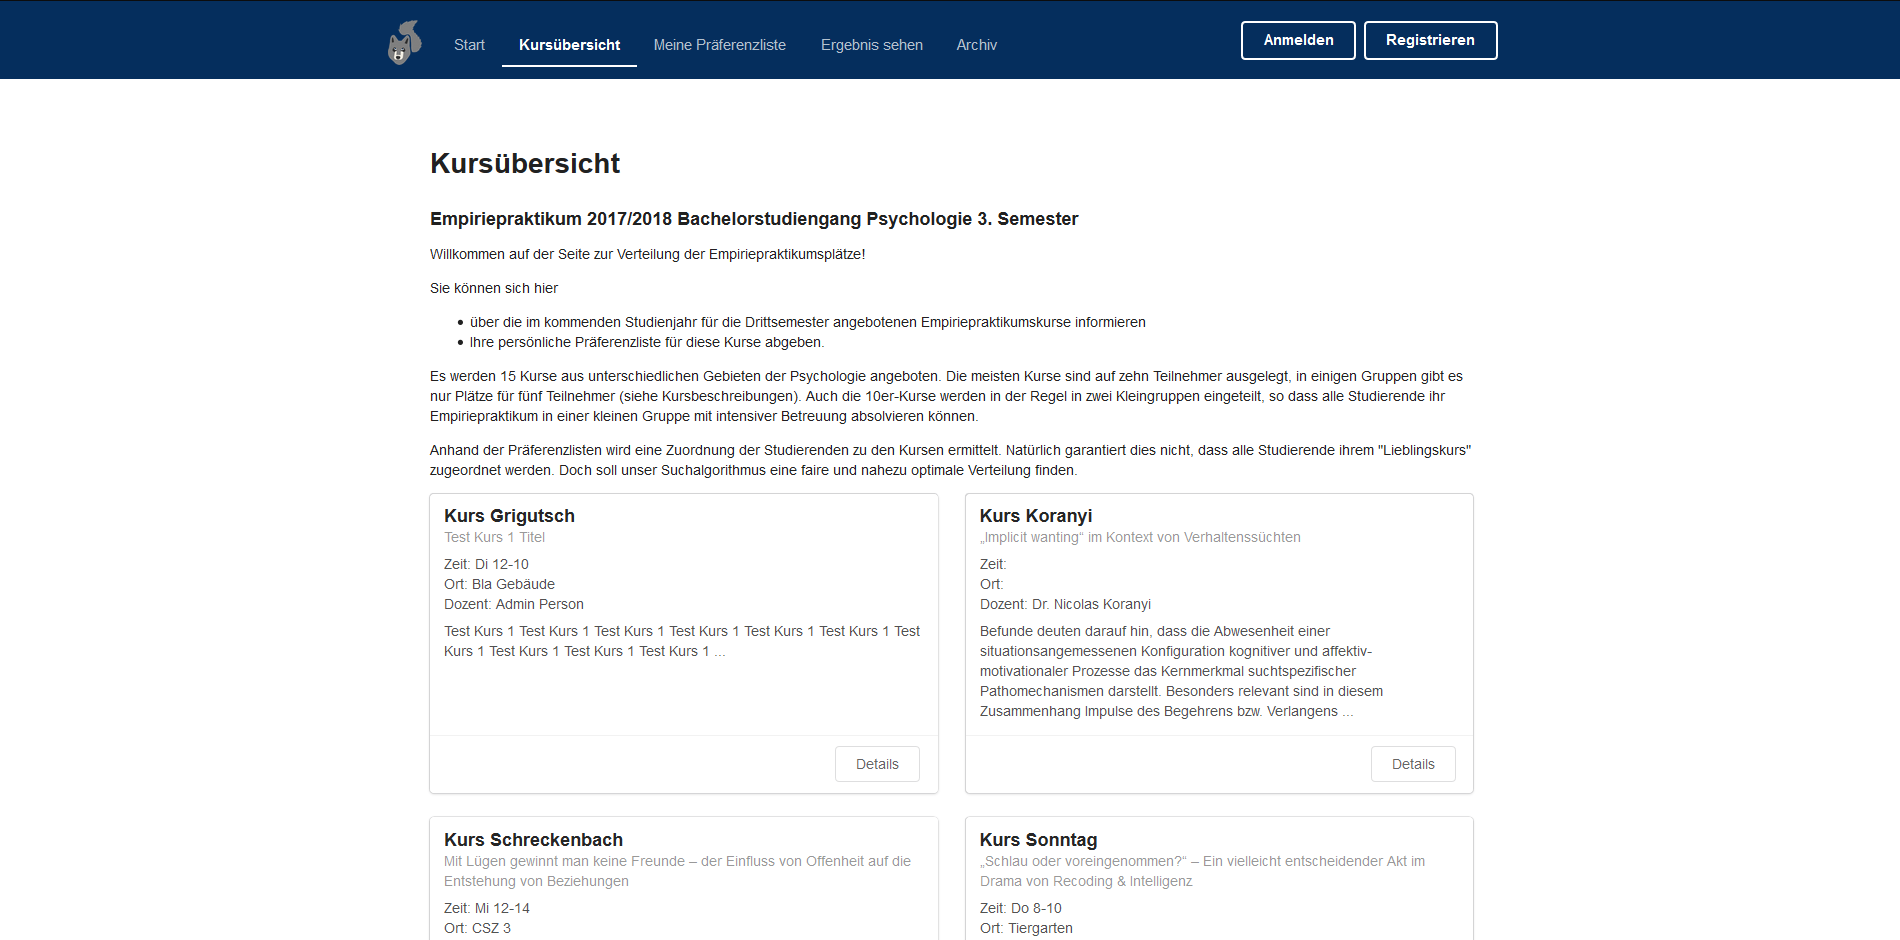
\includegraphics[trim={12cm 5cm 12cm 0},clip,width=1.0\textwidth]{./implementation/images/courses.png}
	            \end{subfigure}
	            \caption{Gegenüberstellung von Entwurf der Kursübersicht und Umsetzung}
	            \label{fig:comparisonCourses}
	        \end{figure}
	    
    
        Abbildung \ref{fig:comparisonCourses} zeigt Entwurf und Umsetzung der Kursübersicht.
        Die Struktur des Entwurfs wurde direkt umgesetzt.
        Wie in Kapitel \ref{chapter:requirements} beschrieben, ist es, wie in Abbildung \ref{fig:comparisonCourses} zu sehen ist, möglich auch ohne eine Anmeldung auf die Kursübersicht zuzugreifen.
        Es ist anzumerken, dass die Fußleiste auch in der Kursübersicht \ref{fig:comparisonCourses} den Abschluss der Seite bildet und lediglich durch die Menge an Kursen nicht zu sehen ist.
        \afterpage{
	        \begin{figure}[p]
	            \centering
	            \begin{subfigure}{0.8\textwidth}
	                \includegraphics[width=1.0\textwidth]{./implementation/images/MockUpsFrontend/frontendPreferences.png}
	            \end{subfigure}
	            \begin{subfigure}{\textwidth}
	                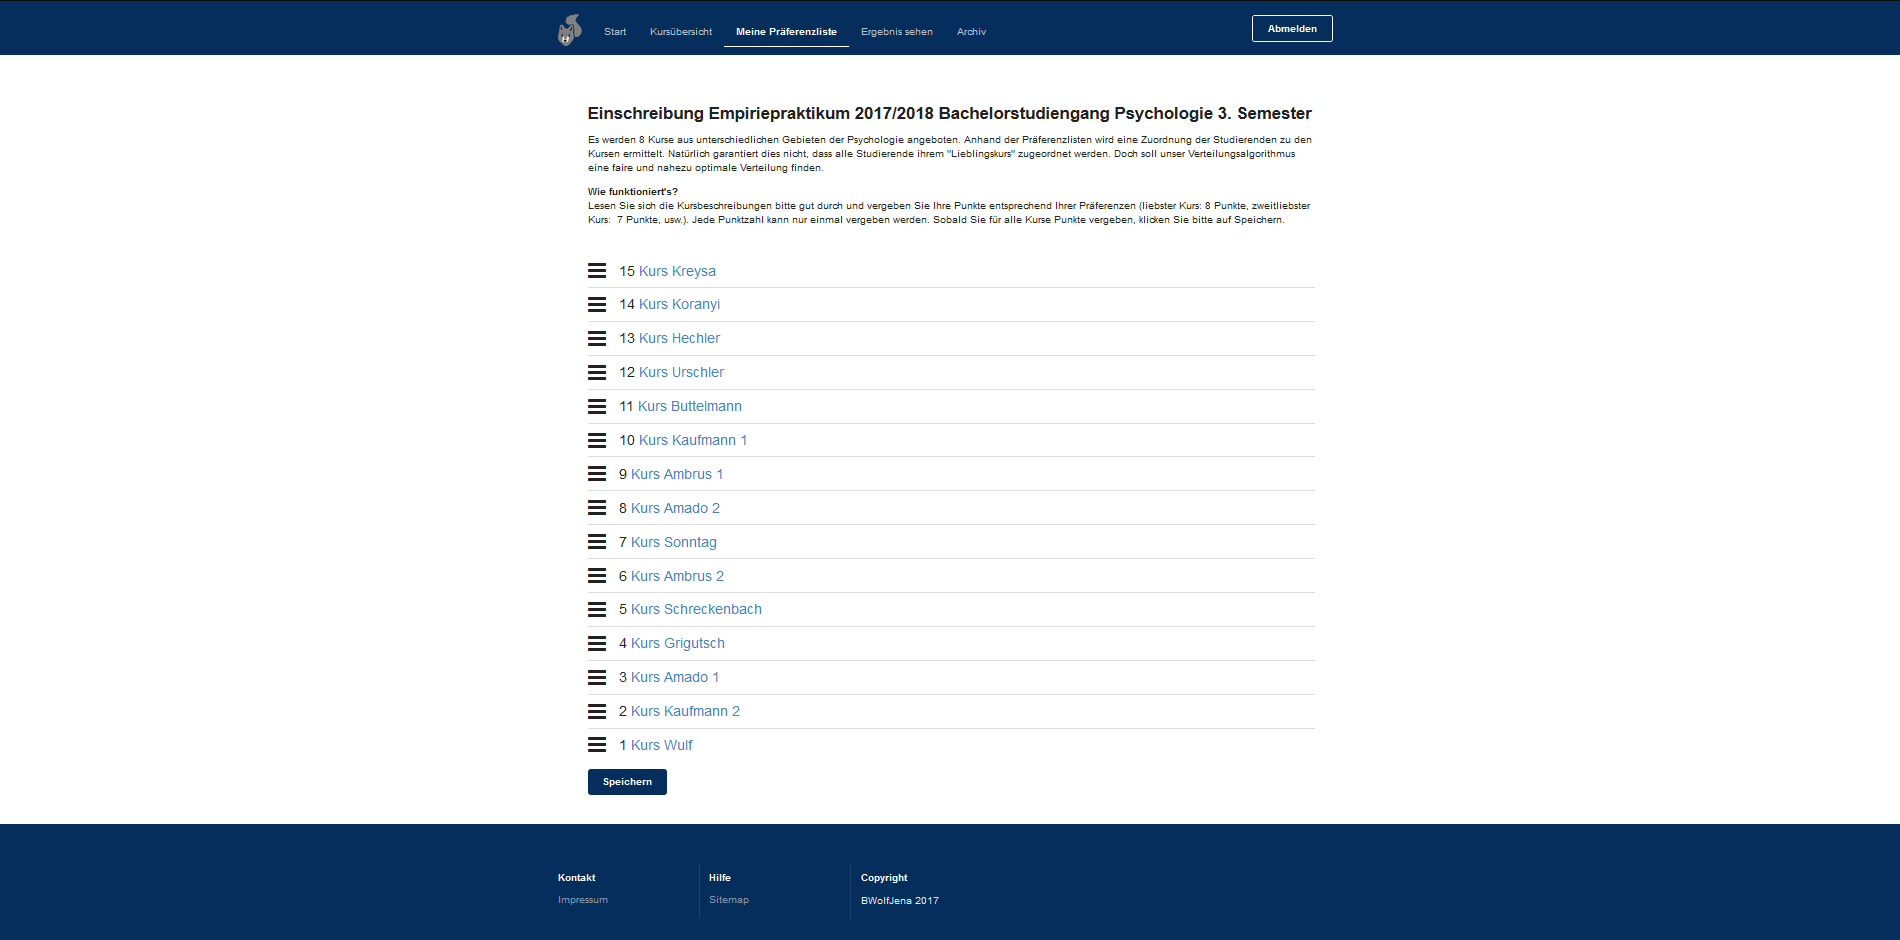
\includegraphics[trim={15cm 0cm 15cm 0},clip,width=\textwidth]{./implementation/images/preferences.png}
	            \end{subfigure}
	            \caption{Gegenüberstellung von Entwurf der Einschreibungs-Oberfläche und Umsetzung}
	            \label{fig:comparisonPrefenrences}
	        \end{figure}
	    }
    
        Die Oberfläche zum Erstellen der Präferenzliste wurde ebenfalls wie angedacht umgesetzt.
        Mithilfe von Drag\&Drop könne die verschiedenen Kurse in die gewünschte Reihenfolge gebracht werden.
        Der Knopf \textit{Absenden} wurde in \textit{Speichern} umbenannt.
        Dadurch soll mehr Klarheit darüber geschaffen werden, dass die Präferenzliste bis zum Ablauf der Frist jederzeit verändert werden kann.\\
        
        Es ist zu erwähnen, dass das gesamte Frontend auch auf mobilen Geräten unterstützt wird.
        Die Ansichten für Kursübersicht und auch die Wahl der Präferenzliste werden entsprechend der Größe des Bildschirms angepasst, sodass die Benutzerfreundlichkeit erhalten bleibt.\\
        
        Die Tauschbörse wurde nicht implementiert.
        Grund hierfür ist zum einen die zeitliche Beschränkung des Projekts, wodurch einige optionale Funktionalitäten nicht umgesetzt werden konnten.
        Zum anderen sind bei einem weiteren Gespräch nach dem Erstellen der Anforderungen Zweifel an der Notwendigkeit solch einer Tauschbörse aufgetreten.
        Eine weitere Funktion, die nicht im Frontend umgesetzt werden konnte, war die in Kapitel \ref{chapter:design} geplante Erweiterbarkeit auf andere Module.
        So kann ein Benutzer im Frontend nicht mehrere Präferenzlisten parallel verwalten.\\
        
        Im Frontend wurde jedoch auch eine zusätzliche Funktionalität implementiert.
        So wurde ein Archiv umgesetzt, in dem die Kurse vergangener Empiriepraktika einsehbar sind.
    
    \section{Backend}
        Auch im Backend ist die Struktur der Entwürfe weitestgehend übernommen worden.
        \afterpage{
	        \begin{figure}[p]
	            \centering
	            \begin{subfigure}{\textwidth}
	                \includegraphics[width=1.0\textwidth]{./implementation/images/MockUpsBackend/backendManageCourses.png}
	            \end{subfigure}
	            \begin{subfigure}{\textwidth}
	                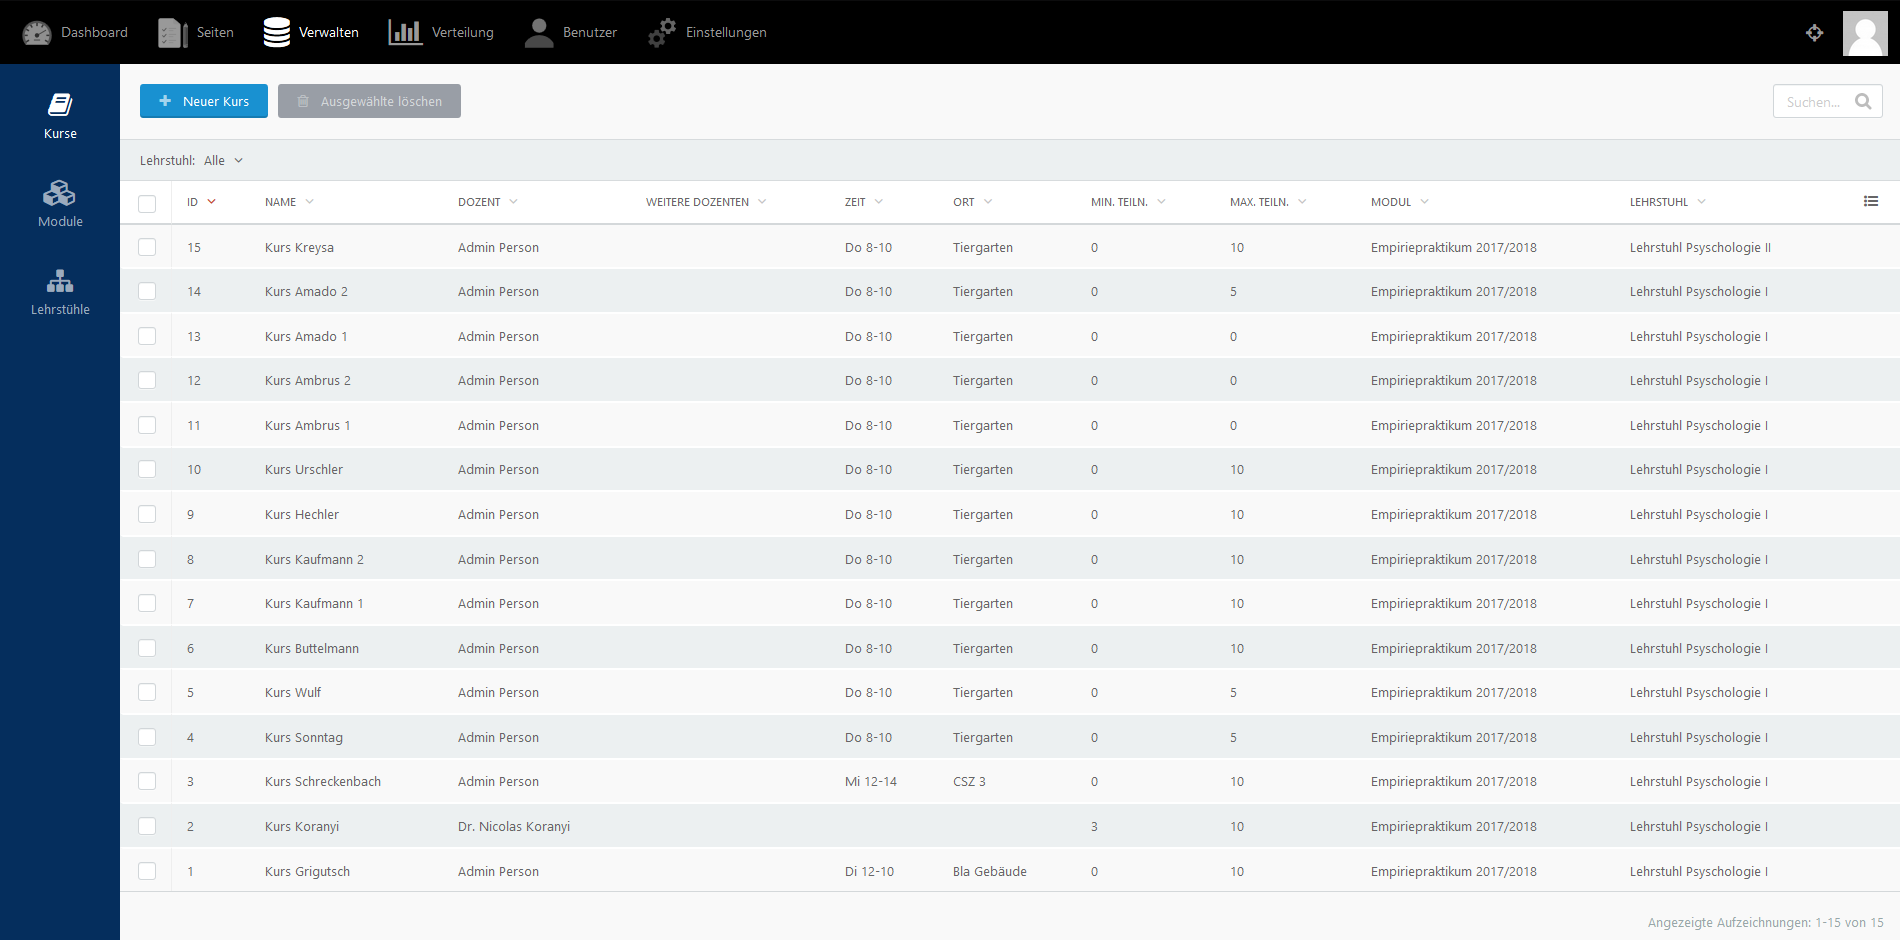
\includegraphics[width=1.0\textwidth]{./implementation/images/manageCourses.png}
	            \end{subfigure}
	            \caption{Gegenüberstellung von Entwurf der Kursverwaltung und Umsetzung}
	            \label{fig:comparisonManageCourses}
	        \end{figure}
	    }
        
        Abbildung \ref{fig:comparisonManageCourses} zeigt Entwurf und Umsetzung der Kursverwaltung.
        Die Struktur aus Kopf- und Seitenleiste wurde übernommen.
        Die Fußzeile wurde jedoch entfernt.
        Es fällt außerdem auf, dass die Kopfzeile mehr Reiter umfasst, als zunächst geplant.
        Das zum Erstellen des Backend verwendete Framework \textit{October CMS} stellt einige vordefinierte Seiten zur Verfügung. Da von Beginn an geplant war für die entsprechenden Funktionen ein CMS zu verwenden wurden dafür keine Mockups erstellt.
        Darunter fällt das \textit{Dashboard}, in dem zum Start des Backends einige wichtige Informationen angezeigt werden.
        Unter dem Reiter \textit{Seiten} können weitere Seiten für das Frontend erstellt und die vorhanden Seiten bearbeitet werden.
        Der Reiter \textit{Einstellungen} ist ebenfalls von \textit{October CMS} bereitgestellt und erlaubt das Ändern und Verwalten verschiedenster Optionen.
        Für dieses Projekt relevant sind vor allem die Einstellungen bezüglich der automatisch versendeten E-Mails, sowie das Verwalten der Backendbenutzer.
        Anders als im Entwurf vorgesehen, werden nicht alle Benutzer über den Reiter \textit{Benutzer} verwaltet, sondern nur die Frontendnutzer.
        Diese Änderung ist durch \textit{October CMS} bedingt.
        
        \begin{figure}[p]
            \centering
            \begin{subfigure}{\textwidth}
                \includegraphics[width=1.0\textwidth]{./implementation/images/MockUpsBackend/backendEdit.png}
            \end{subfigure}
            \begin{subfigure}{\textwidth}
                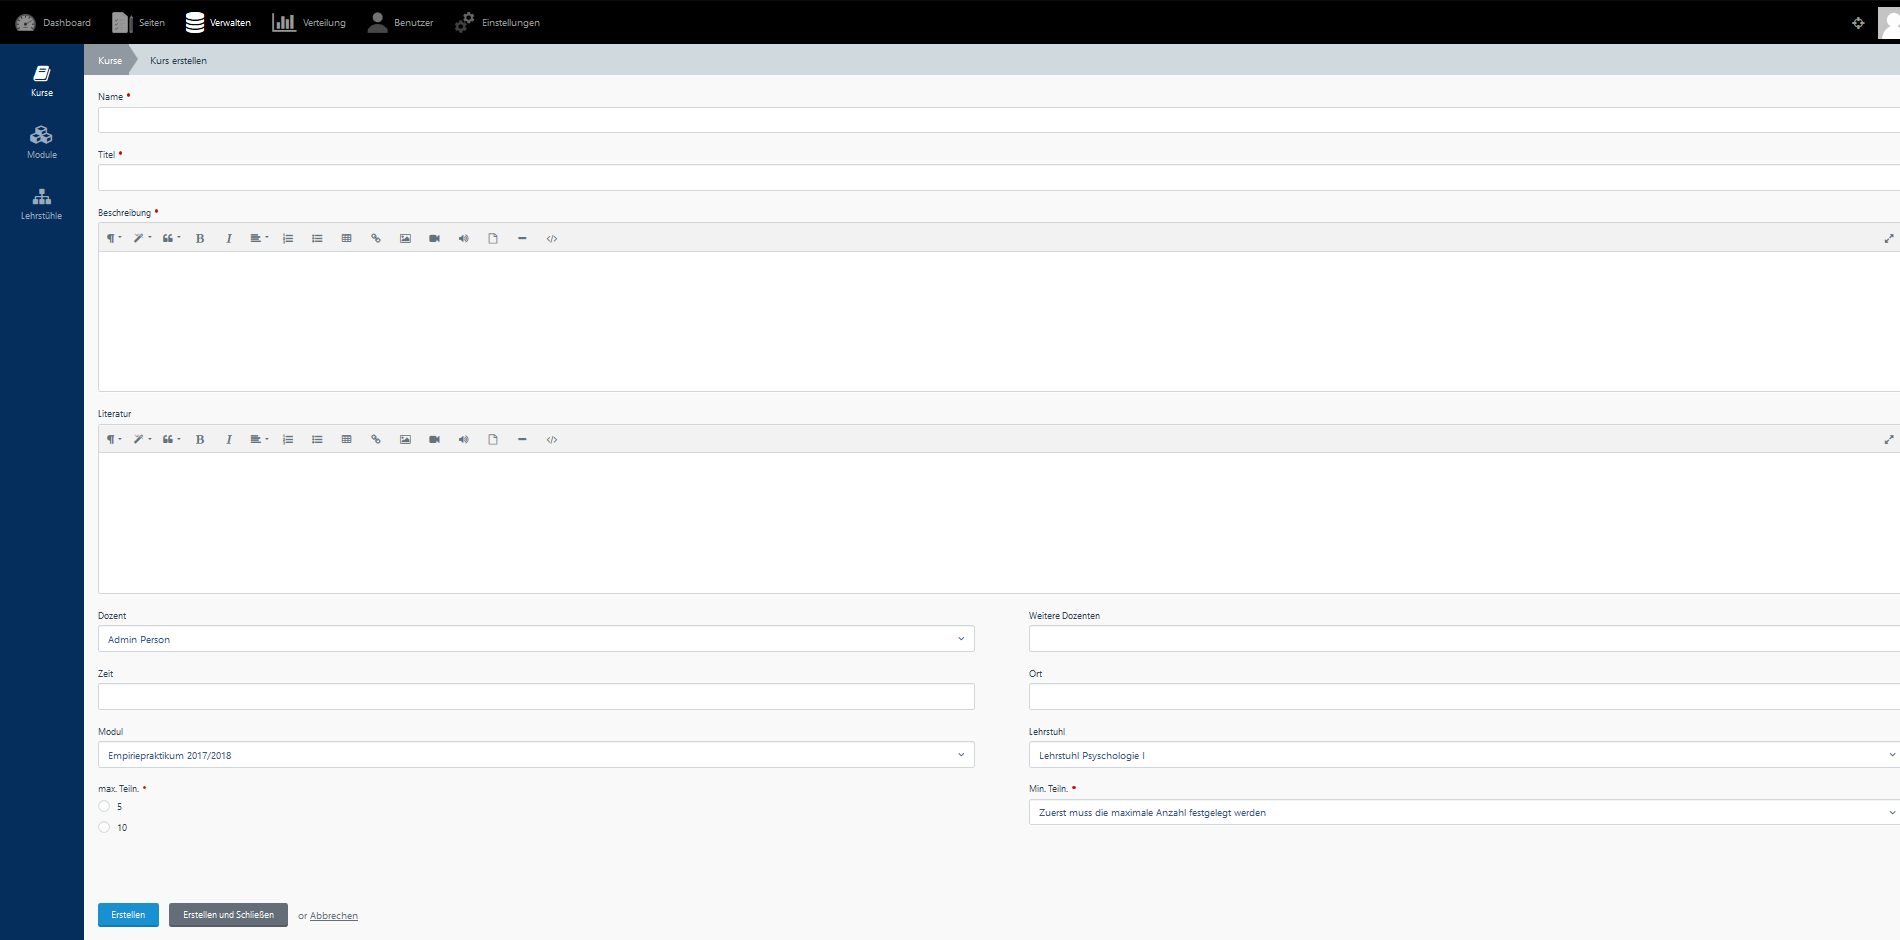
\includegraphics[width=1.0\textwidth]{./implementation/images/edit.png}
            \end{subfigure}
            \caption{Gegenüberstellung von Entwurf der Kurserstellung und Umsetzung}
            \label{fig:comparisonEdit}
        \end{figure}
    
        Das Erstellen und Bearbeiten von Kursen, Lehrstühlen, Benutzern, usw. ist, wie in Abbildung \ref{fig:comparisonEdit} zu sehen, wie im Entwurf umgesetzt.
        Verschiedene Eingabefelder mit \textit{Richtext}-Bearbeitung und Auswahlfelder werden wie vorgesehen zur Verfügung gestellt.
    
        \begin{figure}[p]
            \centering
            \begin{subfigure}{0.9\textwidth}
                \includegraphics[width=1.0\textwidth]{./implementation/images/MockUpsBackend/backendDistribution.png}
            \end{subfigure}
            \begin{subfigure}{\textwidth}
                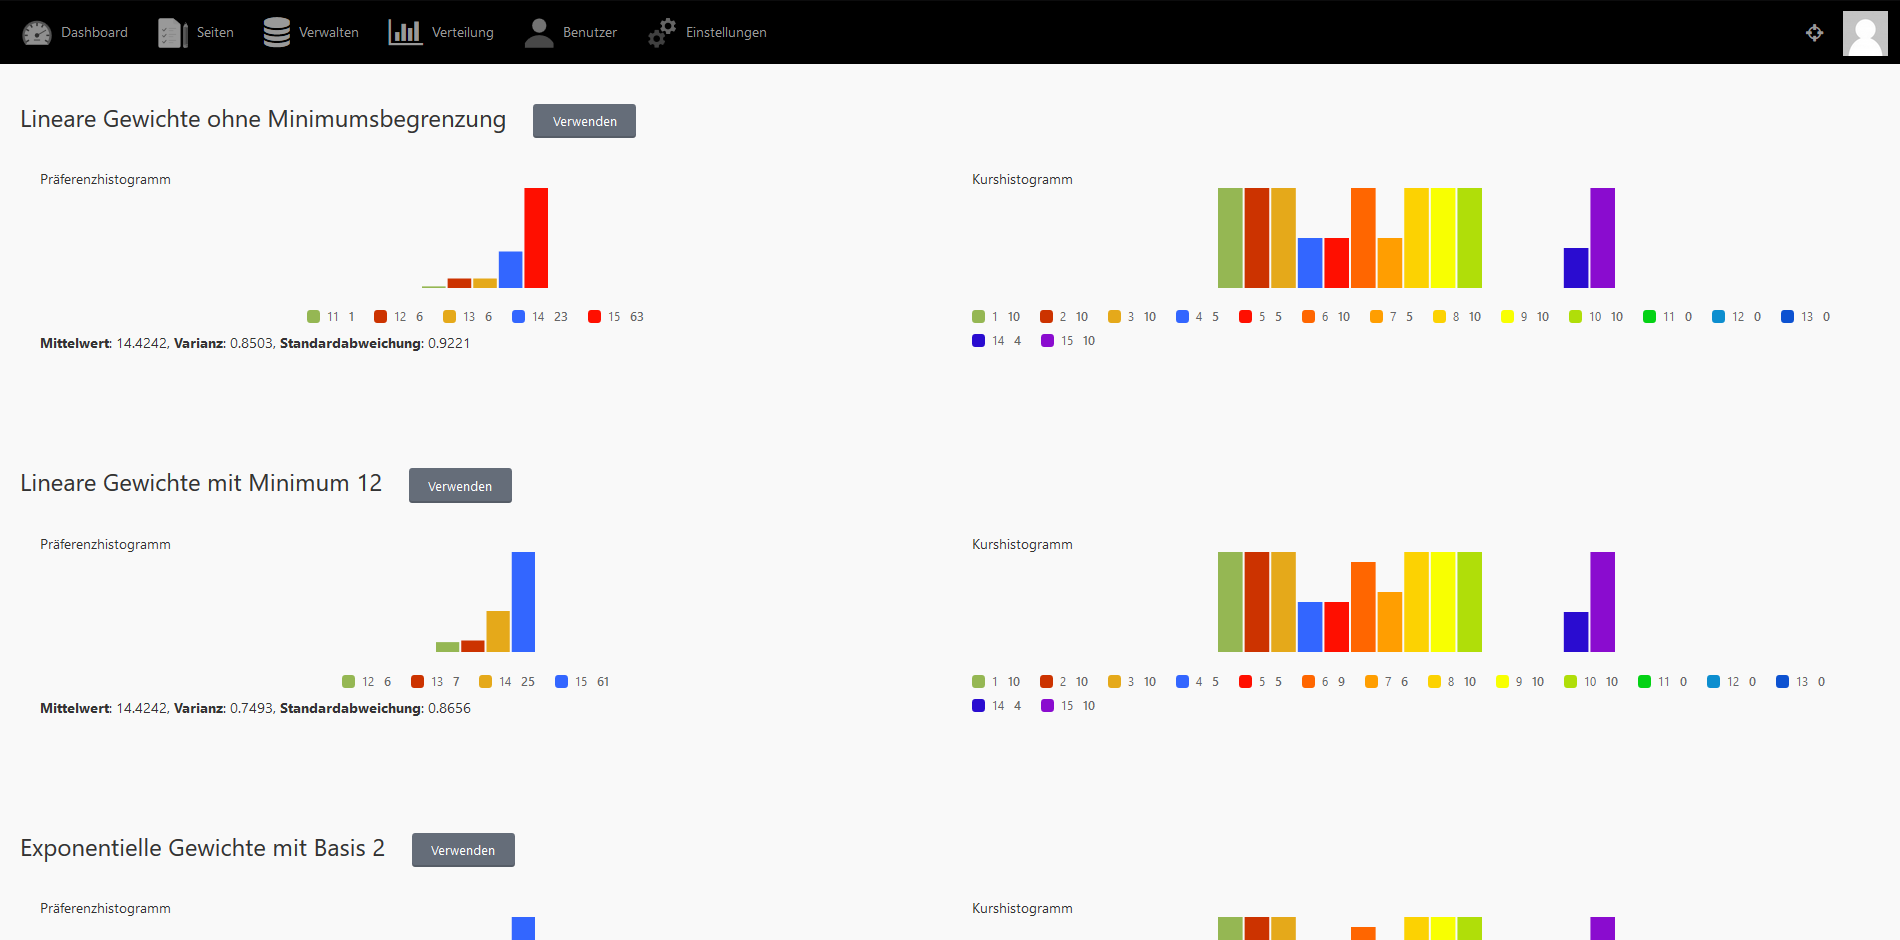
\includegraphics[width=1.0\textwidth]{./implementation/images/distribution.png}
            \end{subfigure}
            \caption{Gegenüberstellung von Entwurf der Anzeige der Verteilungsvorschläge und Umsetzung}
            \label{fig:comparisonDistribution}
        \end{figure}
    
        Auch der Entwurf der Verteilungsansicht wurde umgesetzt.
        In Abbildung \ref{fig:comparisonDistribution} sind wieder Mockup und Resultat gegenübergestellt.
		\pagebreak

    \section{Algorithmus}
	Da lange unbekannt war, ob die für den Algorithmus verwendete Software \textit{lp\_solve}\footnote{\href{http://lpsolve.sourceforge.net/5.5/index.htm}{http://lpsolve.sourceforge.net/5.5/index.htm}} auf dem Server laufen würde, wird der Algorithmus auf einem externen Server ausgeführt. 
    Dazu wurde ein HTTP-Service in \textit{Node.js} implementiert, der eine Liste mit Kursteilnehmerbegrenzungen, die Präferenzlisten (nur IDs), sowie die Parameter für den Algorithmus (minPref, weights) entgegennimmt und mit der Lösung des in Kapitel \ref{chapter:algorithm} beschriebenen Optimierungsproblems antwortet.	
    Da es kein Budget für das Projekt gab, wird der Server dauerhaft kostenlos bei \textit{Heroku} \footnote{\href{https://www.heroku.com/home}{https://www.heroku.com/home}} gehostet. 
    Nach 30 Minuten Inaktivität geht er dabei in den Ruhezustand wodurch die nächste Anfrage ein paar Sekunden langsamer beantwortet wird. 
    Falls \textit{Heroku} diesen Service einstellen sollte, kann der Algorithmus auch lokal ausgeführt werden. 
    Eine Anleitung wie die lokale Umgebung installiert wird befindet sich in der Anwenderdokumentation. 
    Die Daten müssen dann mit Hilfe eines \textit{MySQL} Clients vom Server der Universität exportiert und lokal importiert werden. 
    Zum Exportieren und Importieren von Daten befindet sich ebenfalls ein Abschnitt in der Anwenderdokumentation. 
    
    
    
    
    

    \section{Überlegungen zum Algorithmus}
        Die Grundlegende Idee der Zielfunktion hat die Form:
            $$ \max ~\text{Summe der Prioritäten} - \text{Gewicht} \cdot \text{Varianz} ~~~.$$
        Genauer ausformuliert ergibt sich:
            $$ \max 
                \sum_{i=1}^{n} \sum_{j=1}^{m} c(i,j)x_{ij} 
                - \frac{\beta}{n} \sum_{i=1}^{n}
                    \left[\left(\sum_{i=1}^{m} c(i,j)x_{ij}\right) - \frac{1}{n} \sum_{i=1}^{n} \sum_{j=1}^{m} c(i,j)x_{ij}\right] ~~~,$$
        wobei gilt:\\
            \begin{tabular}{l c l}
                $n$ & - & Anzahl der Studenten \\
                $m$ & - & Anzahl der Kurse\\
                $ c(i,j) $ & - & Priorität von Student $ i $ für Kurs $ j $\\
                $ \beta $ & - & Gewichtung der Varianz\\
                $t_{\min}(j)$ & - & Minimale Anzahl der Teilnehmer für Kurs $ j $\\
                $t_{\max}(j)$ & - & Maximale Anzahl der Teilnehmer für Kurs $ j $ ~~~.\\
            \end{tabular}\\
        
        Zusätzlich sind drei Nebenbedingungen notwendig, um das Problem angemessen darzustellen.
        Zum einen sollen die $ x_{ij} $ nur die Werte 0 oder 1 annehmen können:
            $$ x_{ij} \in \{0,1\} ~~~.$$
        Des Weiteren soll jeder Student nur einem Kurs zugeteilt werden:
            $$ \forall {i \in \{1,..,n\}}: \sum_{j=1}^{m} x_{ij} = 1 ~~~.$$
        Zuletzt ist die Teilnehmerzahl für die Kurse begrenzt:
            $$ \forall {j \in \{1,..,m\}}: t_{\min}(j) \leq \sum_{i=1}^{n} x_{ij} \leq t_{\max}(j) ~~~.$$
    \section{Stand des Projekts}

\section{Offene Probleme}

\section{Mögliche weitere Arbeiten}
    \clearpage
\chapter{Anhang}
\label{chapter:appendix}
%    \section{Anhang - Entwurf}
%        \begin{figure}[t]
%            \centering
%            \includegraphics[width=0.7\textwidth]{./design/images/MockUpsFrontend/frontendRegistration.png}
%            \caption{Entwurf für Registrierungs-Oberfläche}
%            \label{fig:mockupRegistrationFrontend}
%        \end{figure}
%        
%        \begin{figure}[t]
%        	\centering
%        	\includegraphics[width=0.7\textwidth]{./design/images/MockUpsFrontend/frontendCoursedetails.png}
%        	\caption{Entwurf für die Kursdetails}
%        	\label{fig:mockupDetailsFrontend}
%        \end{figure}
%    
%        \begin{figure}[t]
%        	\centering
%        	\includegraphics[width=0.7\textwidth]{./design/images/MockUpsFrontend/frontendResults.png}
%        	\caption{Entwurf für die Ergebnisübersicht}
%        	\label{fig:mockupResultsFrontend}
%        \end{figure}
%    
%        
    
    
    
\end{document}